\subsection{Test HTTP Methods - OTG-CONFIG-006}

\begin{longtable}[l]{ p{2.3cm} | p{.79\linewidth} }\hline
    & \textbf{InternetBanking} \\ \hline
    \textbf{Observation} & It was found that there is no reference to methods other than GET and POST, in the source code. \\
    \textbf{Discovery} & The PHP source code was examined using \code{grep} command and this was confirmed using the Nmap tool which revealed that the server allows only 4 methods : HEAD, GET, POST, OPTIONS. See Figure \ref{fig:nmap_http_methods}. \\
    \textbf{Likelihood} & N/A \\
    \textbf{Impact} & N/A \\
    \textbf{Recommen\-dations} & N/A \\ \hline
    \textbf{CVSS} & N/A
    \\ \hline
\end{longtable}

\subsubsection{SecureBank}
\begin{longtable}[l]{ p{2.3cm} | p{.79\linewidth} }\hline
    & \textbf{SecureBank} \\ \hline
    \textbf{Observation} & It was found that there is no reference to methods other than GET and POST, in the source code. \\
    \textbf{Discovery} & The PHP source code was examined using \code{grep} command. \\
    \textbf{Likelihood} & N/A \\
    \textbf{Impact} & N/A \\
    \textbf{Recommen\-dations} & recommendations \\ \hline
    \textbf{CVSS} & N/A
    \\ \hline
\end{longtable}

\subsubsection{Comparison}
Both applications exhibit similar behavior with respect to the allowed HTTP methods and neither contain any vulnerabilty.
\\
\begin{figure}[ht]
	\centering
		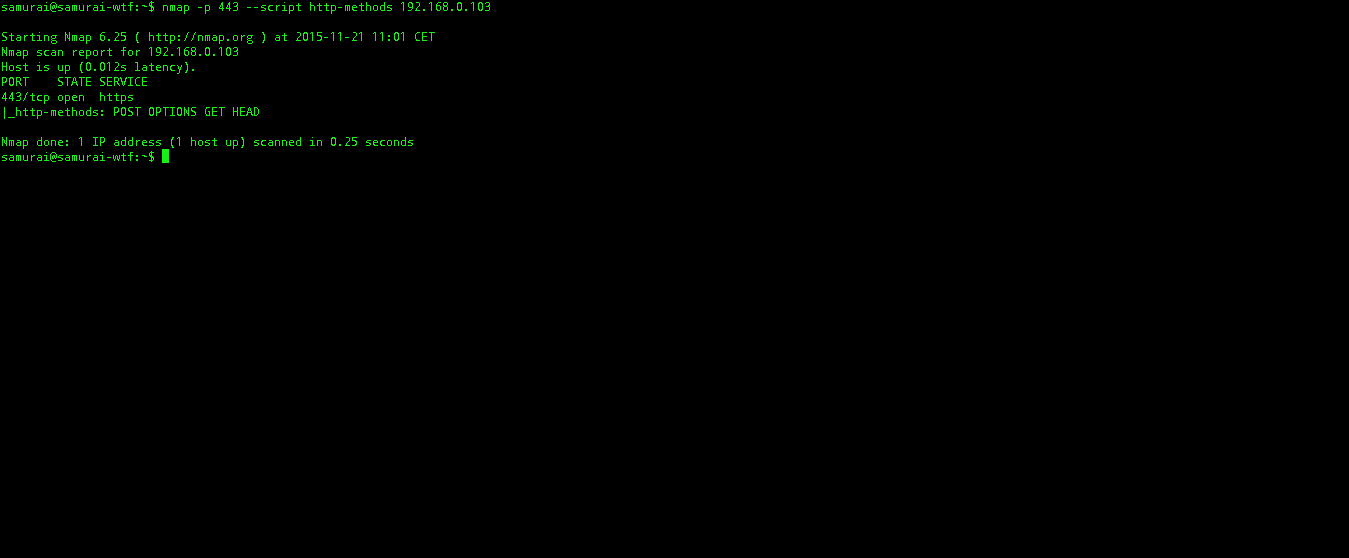
\includegraphics[width=.8\linewidth]{figures/OTG-CONFIG-006.png}
		\caption{Nmap - Check for allowed HTTP methods}
	\label{fig:nmap_http_methods}
\end{figure}

\clearpage